\section{Signal}
\label{sec:signal}
This analysis searches for the simultaneous production of two massive bosons and a photon in a single hard scattering of a proton-proton collision at 13\TeV.
The signature of these processes varies among the three channels, but includes a number of high-momentum, isolated leptons,
with one or two pairs resonating to the Z boson mass,
and an isolated photon with high momentum.

However, there is a degree of ambiguity in what can be considered triboson production when a photon is present in the final state.
For example, in the four lepton channel, the reaction
$p p \to 4 \Pl \PGg$
has three contributions:
\begin{enumerate}
\item The photon comes from an initial state fermion (Figure \ref{fig:ppTo4LG_hard})
\item The photon comes from a Triple or Quartic Gauge Coupling (e.g. Figure \ref{fig:ppTo4LG_GC})
\item The photon is emitted as Final State Radiation (FSR) by one of the leptons from the decay of a \PZ (e.g. Figure \ref{fig:ppTo4LG_FSR})
\end{enumerate}
Arguably only the first and second process are strictly considerable triboson production.

The goal of this analysis is to measure both the inclusive cross sections
$\sigma(pp \to 4\Pl \PGg)$, $\sigma(pp \to 3\Pl \PGnl \PGg)$ and $\sigma(pp \to 2\Pl 2j \PGg)$
and the significance of triboson production in the same channels.
Therefore a dedicated cut, described in Section \ref{sec:FSR_cut}, was devised to exclude events in which
the (genuine) photon comes from final state radiation,
and results are derived both with (triboson fiducial region) and without (inclusive cross section) applying it.

It is worth noting that in the SM only $\PW\PZ\PGg$ can be produced via triple and quartic gauge couplings,
while $\PZ\PZ\PGg$ does not have any leading order (perturbative expansion up to $\alpha_{EW}^6$) contribution from TGC nor QGC.

\begin{figure}
  \centering
  \subfigure [From initial-state fermion] {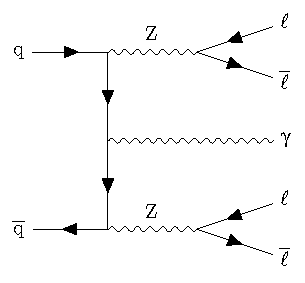
\includegraphics[width=.319\textwidth]{triboson_4LG.pdf} \label{fig:ppTo4LG_hard}}
  \subfigure [Non-abelian coupling]       {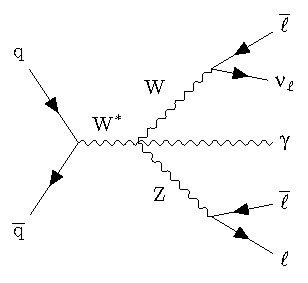
\includegraphics[width=.319\textwidth]{QGC_3LNuG.pdf}    \label{fig:ppTo4LG_GC}  }
  \subfigure [From final-state fermion]   {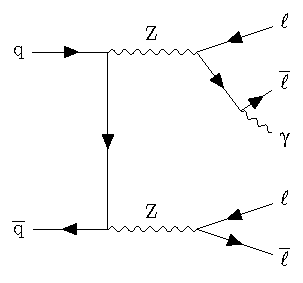
\includegraphics[width=.319\textwidth]{ZZ_4LG.pdf}       \label{fig:ppTo4LG_FSR} }
\caption{Representative Standard Model Feynman diagrams that yield four isolated leptons and a photon in the final state.}
\label{fig:ppTo4LG}
\end{figure}
